\chapter{Introducción}
\label{section:intro}

El presente trabajo tiene como objetivo principal el desarrollo de un sistema de comunicaciones basado en 16-QAM (Modulación de Amplitud en Cuadratura de 16 niveles). Para ello, se propone el empleo en conjunto de los diferentes bloques electrónicos IP estudiados en la asignatura y se divide el desarrollo del entregable en una serie de fases de configuración:

\vspace{1mm}

\begin{itemize}
    \item \textbf{Captura XADC y Memoria FIFO:} En esta primera etapa se realizará la captura de una señal triangular y se procederán a almacenar los datos de entrada en una memoria FIFO.
    \item \textbf{Modulador 16-QAM:}
        \begin{itemize}
            \item \textbf{Mapeado QAM y Zero Padding: } Como siguiente paso a seguir, se generará el mapeado de 16-QAM y se implementará un Zero-Padding 1:32. 
            \item \textbf{Filtrado Root Raised Cosine: } Tras aplicar Zero Padding, se deberá generar y aplicar a cada rama I/Q el filtrado pulse shaping del “root raised cosine” (RRC).
            \item \textbf{Mezclador DDS y Multiplicadores: ----------}
            \item \textbf{Sumador: ----------}
            \item \textbf{Rx: ----------}
        \end{itemize}
    
\end{itemize}

\vspace{3mm}

    \begin{figure}[h]
    	\centering
    	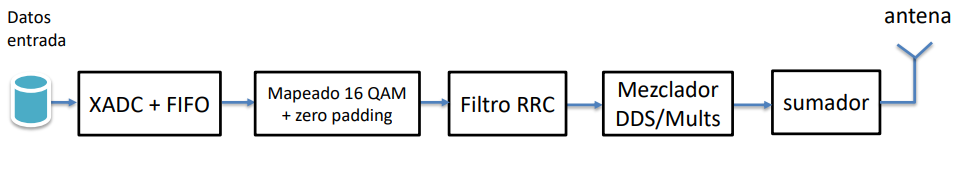
\includegraphics[width=1\textwidth]{img/diseno/sistema.PNG}
    	\caption{Distribución de bloques del sistema de comunicaciones}
    	\label{fig:sistema}
    \end{figure}
    
\vspace{3mm}

Para lograr tanto un correcto funcionamiento de cada bloque electrónico como la interoperabilidad entre ellos al integrarlos en del sistema, será preciso un estudio en profundidad de la documentación proporcionada por el fabricante y un análisis cuantitativo y cualitativo de cada uno de los resultados obtenidos en las simulaciones funcionales. 

\vspace{1mm}

%Finalmente, se deberá evaluar la eficacia de la modulación 16-QAM en la transmisión de datos
%Se adjunta el enunciado en archivo pdf y un archivo de matlab "qam16.m" para simular el funcionamiento de la transmisión de datos usando 16QAM.


%1.	Obtención de los datos convertidos del ADC – simulación señal de entrada 
%2.	Lógica de control de lectura/escritura de los datos de la FIFO. Comprobación del bloque FIFO 

%3.	Bloque de mapeado 16QAM y zero-padding 
%4.	Bloque de filtrado pulse shaping - RRC 
%5.	Generación de las sinusoides coseno/-seno mediante bloque DDS a 576 MHz 

%6.	Bloque de multiplicación y suma de señales de transmisión I/Q. Comprobación de datos. 
%7.	Configuración y uso del bloque MMCM en el diseño

%8.	Codificación de ficheros testbench y pruebas realizadas para la verificación del funcionamiento junto con el simulador Matlab. 
%9. Realización de un diseño modular que funcione correctamente en su conjunto 
%10. Inclusión de otras alternativas/opciones adicionales en el diseño planteado





